\subsection{The classifier stage}

After being proposed by the previous stage, in this stage, proposed regions are examined more carefully using other algorithms.
To classify these object, we don't usually use the pixels directly. The two popular methods are appearance-based method and feature-based method. 
Appearance based method uses example images to perform this stage, but changes in lighting or color, changes in view direction, and changes in size or shape can fail our system. Edge matching, greysacle matching and gradient matching are some of appearance-based methods.

The other method is feature-based method. In this method, we usually extract some features from objects to use instead of using the pixels directly.\cite{realtimeface}. The reason they explained in \cite{realtimeface} is because feature an act to encode ad-hoc domain knowledge that is difficult to learn using a finite quantity of data and the feature based system operates much faster than a pixel based system. There are a lot of feature we can use. 

In face detection\cite{realtimeface}, Paul and Michael use Rectangle feature. \\
\begin{figure}
	\centering
	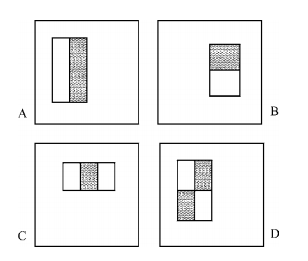
\includegraphics[width = 0.5\textwidth]{rectangleFeature}
	\caption{Example rectangle features shown relative to the enclosing detection window. The sum of the pixels which lie within the white rectangles are ubtracted from the sum of pixels in the grey rectangles \cite{realtimeface}}
\end{figure}
Them sum of pixels which lie within the white rectangles are substracted from the sum of pixels in the grey rectangles. Using intergral image \cite{realtimeface}, we can compute any rectangle feature rapidly. Other popular feature we can use are SIFT, SURF, HOG, etc.